\chapter{Прикладная аэродинамика паруса}\label{chap:2}

\section{Работа паруса}

Современная теория паруса основывается на положениях аэродинамики крыла, элементы которой были рассмотрены в главе <<Элементы теории парусной яхты>> (см. <<Сопротивление дрейфу>>). Механика возникновения аэродинамической силы на парусе, изготовленном из ткани, в принципе аналогична и для жёсткого профилированного крыла. В любом поперечном сечении паруса должна развиться циркуляция потока воздуха, как вокруг профиля крыла (см. рис.~\ris{8}), чтобы появилась подъёмная сила.

Естественно, что аэродинамика паруса из ткани имеет ряд существенных отличий от жёсткого крыла, каким, например, является яхтенный киль. Вследствие эластичности ткани парус изменяет свой профиль под влиянием потока воздуха. Он обладает способностью скручиваться \--- изменять угол атаки по отношению к ветру по высоте. В отличие от получивших распространение аэродинамических профилей со сравнительно толстой входящей кромкой парус имеет острую переднюю кромку и выпукло\-/вогнутую форму, образованную тонким материалом. Наконец, передней кромкой парус может крепиться к мачте, имеющей довольно большое поперечное сечение, что вносит существенное изменение в картину обтекания паруса потоком и в распределении давления по ширине паруса.

\begin{figure}[htb]
  \centering
  \includegraphics[scale=1.2]{0019P.pdf}
  \caption{Схема сил, действующих на паруса яхты; основные угловые параметры движения и установки парусов}
  \label{fig:19}
  \centering{}
  \small
  $\beta$ \--- путь яхты по отношению к вымпельному ветру; $\lambda$ \--- угол дрейфа; $\alpha$ \--- угол атаки паруса; $\delta$ \--- угол установки паруса относительно \textit{ДП} яхты; \vidx{V}{И} \--- скорость истинного ветра; \ve V \--- скорость яхты; \vidx{V}{В} \--- скорость вымпельного ветра; \vidx{V}{НВ} \--- скорость прямо против ветра
\end{figure}

Наиболее важные элементы, влияющие на аэродинамику паруса, будут рассмотрены дальше, но для начала установим влияние составляющих аэродинамической силы на движение яхты при различных курсах относительно ветра.

Если яхта идёт курсом бейдевинд, то под действием набегающего потока воздуха на парусах, установленных под углом атаки $\alpha$ к направлению вымпельного ветра, возникает результирующая аэродинамическая сила \ve A (рис.~\ris{19}). По аналогии с жёстким крылом эту силу можно разложить на две составляющие: подъёмную силу \ve Y, перпендикулярную направлению вымпельного ветра, и лобовое сопротивление \ve X, действующее по направлению ветра. В дальнейшем эти силы мы будем использовать для рассмотрения характеристик паруса и всего парусного вооружения в целом. 

Для того чтобы оценить влияние аэродинамической силы \ve A на движение яхты, представим её в виде двух других составляющих: силы тяги \ve T, направленной по оси движения судна, и перпендикулярной ей силы дрейфа \ve D. Направление движения яхты (путь) отличается от её курса на величину угла дрейфа $\lambda$, однако в дальнейшем анализе этим углом можно пренебречь. 

Предположим, что на выбранном курсе бейдевинд удалось увеличить подъёмную силу на парусе до величины \vidx{Y}{1}, а лобовое сопротивление не изменилось. Силы \vidx{Y}{1} и \ve X, будучи сложенными по правилу сложения векторов, образуют новую аэродинамическую силу \vidx{A}{1}. Изменятся и её составляющие относительно оси движения яхты \ve T и \ve D. Без вычислений можно сказать, что в данном случае с увеличением подъёмной силы увеличатся и сила тяги, и сила дрейфа (рис.~\ris{20}). Аналогичное построение позволяет убедиться, что при увеличении лобового сопротивления на курсе бейдевинд сила тяги уменьшается, а сила дрейфа увеличивается. Таким образом, при плавании в лавировку экипаж яхты должен стремиться по возможности добиться образования на парусах максимальной подъёмной силы при минимальной величине лобового сопротивления. Иными словами, для острых курсов необходима работа паруса с максимальным аэродинамическим качеством, которое численно выражается в отношении подъёмной силы к лобовому сопротивлению. 

\begin{equation}
\ve K = \ve Y / \ve X
\end{equation}

Отметим, что на курсе бейдевинд вымпельный ветер, являющийся результатом сложения векторов истинного ветра и движения яхты, имеет наивысшую скорость \vidx{V}{В} (см. рис.~\ris{19}, \textit{б}), что сказывается на величине обеих составляющих аэродинамической силы \--- \ve Y и \ve X.

На курсе галфвинд подъёмная сила является силой тяги, а лобовое сопротивление \--- силой дрейфа. Если лобовое сопротивление увеличить, то увеличится только сила дрейфа. Однако на ходовые качества яхты это влияет в заметно меньшей степени, чем на курсе бейдевинд, поскольку скорость вымпельного ветра на курсе галфвинд снизилась и, следовательно, величина силы дрейфа меньше.

\begin{figure*}[htb]
  \centering
  \includegraphics[scale=1.3]{0020P}
  \caption{Роль составляющих аэродинамической силы на различных курсах относительно вымпельного ветра}
  \label{fig:20}
\end{figure*}

На курсе бакштаг парус работает на больших углах атаки, при которых подъёмная сила оказывается значительно меньше лобового сопротивления. Если увеличить лобовое сопротивление, то тяга и сила дрейфа увеличатся. При возрастании подъёмной силы тяга также увеличивается, а сила дрейфа уменьшается. Следовательно, на курсе бакштаг рост и подъёмной силы и (или) лобового сопротивления увеличивает тягу. Сила дрейфа тем больше, чем больше лобовое сопротивление. На курсе фордевинд угол атаки паруса близок к 90\gr, поэтому подъёмная сила на парусе равна нулю, а лобовое сопротивление направлено по оси движения яхты и становится силой тяги. Сила дрейфа равна нулю. Следовательно, на курсе фордевинд для увеличения силы тяги нужно увеличивать лобовое сопротивление парусного вооружения, что на гоночных яхтах достигается постановкой дополнительных парусов \--- \textbf{спинакера} и \textbf{блупера}, имеющих большую площадь и плохо обтекаемую форму. 

Отметим, что на курсе фордевинд на паруса действует вымпельный ветер минимальной скорости, в результате чего на паруса действуют сравнительно умеренные силы.

\section{Особенности работы паруса как крыла}

Только при небольшом значении угла атаки, когда на остром и тонком профиле ещё не образуется подъёмная сила, парус обтекается потоком воздуха, одинаково плавным с нижней и с верхней стороны. При небольшом увеличении угла атаки критическая точка перемещается на нижнюю сторону профиля и потоку приходится огибать острую кромку с большой скоростью. В результате у входящей кромки образуется значительное разрежение и под влиянием этого разрежения пограничный слой отрывается от поверхности профиля, образуя на его спинке вихревой пузырь. При достаточно большой скорости ветра поток быстро поглощает энергию вихрей и слой вновь  присоединяется к поверхности профиля на некотором расстоянии от входящей кромки (рис.~\ris{21}).

\begin{figure*}[htb]
  \centering
  \includegraphics[scale=1.3]{0021P}
  \caption{Режим обтекания паруса и распределение пониженного давления (разрежения) по ширине профиля в зависимости от угла атаки $\alpha$}
  \label{fig:21}
\end{figure*}

Вихревой пузырь, размеры которого увеличиваются по мере увеличения угла атаки, вносит существенные изменения в распределение пониженного давления вдоль подветренной стороны паруса по сравнению с показанным на рис.~\ris{10} распределением давления на жёстком профиле с толстой скруглённой передней кромкой. Напомним, что именно разрежение на подветренной стороне паруса играет основную роль в создании подъёмной силы и, следовательно, силы тяги на острых к ветру курсах. 

На рис.~\ris{21} представлены результаты замеров разрежения на жёстком выпукло-вогнутом профиле, аналогично парусу. На малых углах атаки профиль обтекается плавным ламинарным потоком. 

При $\alpha = 4\gr$ начинаете отрыв пограничного слоя. В этот момент достигается наивысшее разрежение, пик которого расположен вблизи входящей кромки.
 
При $\alpha = 6\gr$ вихревой пузырь занимает на подветренной стороне около 25\,\% хорды профиля $b$. Разрежение уменьшается, и эпюра его становится более плавной. 

При $\alpha = 10\gr$ пузырь охватывает всю ширину профиля, его толщина составляет 3,5\,\% $b$. Давление повышается в 2,5 раза по сравнению с разрежением при $\alpha = 4\gr$; пика разрежения практически нет \--- оно равномерно распределено по всей ширине профиля. Значит, подъемная сила существенно снизилась, а лобовое сопротивление возросло (см. рис.~\ris{27}). 

Таким образом, на курсе бейдевинд увеличение угла атаки паруса к вымпельному ветру более 5\otdo 6\gr нежелательно. На реальном парусе вихревой пузырь представляет собой невидимый глазу цилиндрический валик, распространяющийся по всей высоте паруса. Чем больше выбран шкот, тем большая часть подветренной поверхности паруса захватывается вихревым валиком, уменьшая подъёмную силу. 

Для выбора оптимального угла атаки в последние годы используются индикаторы обтекания в виде ленточек из тонкой ткани, закреплённых на определённом расстоянии от передней шкаторины с обеих сторон паруса (рис.~\ris{22}).

\begin{figure*}[htb]
  \centering
  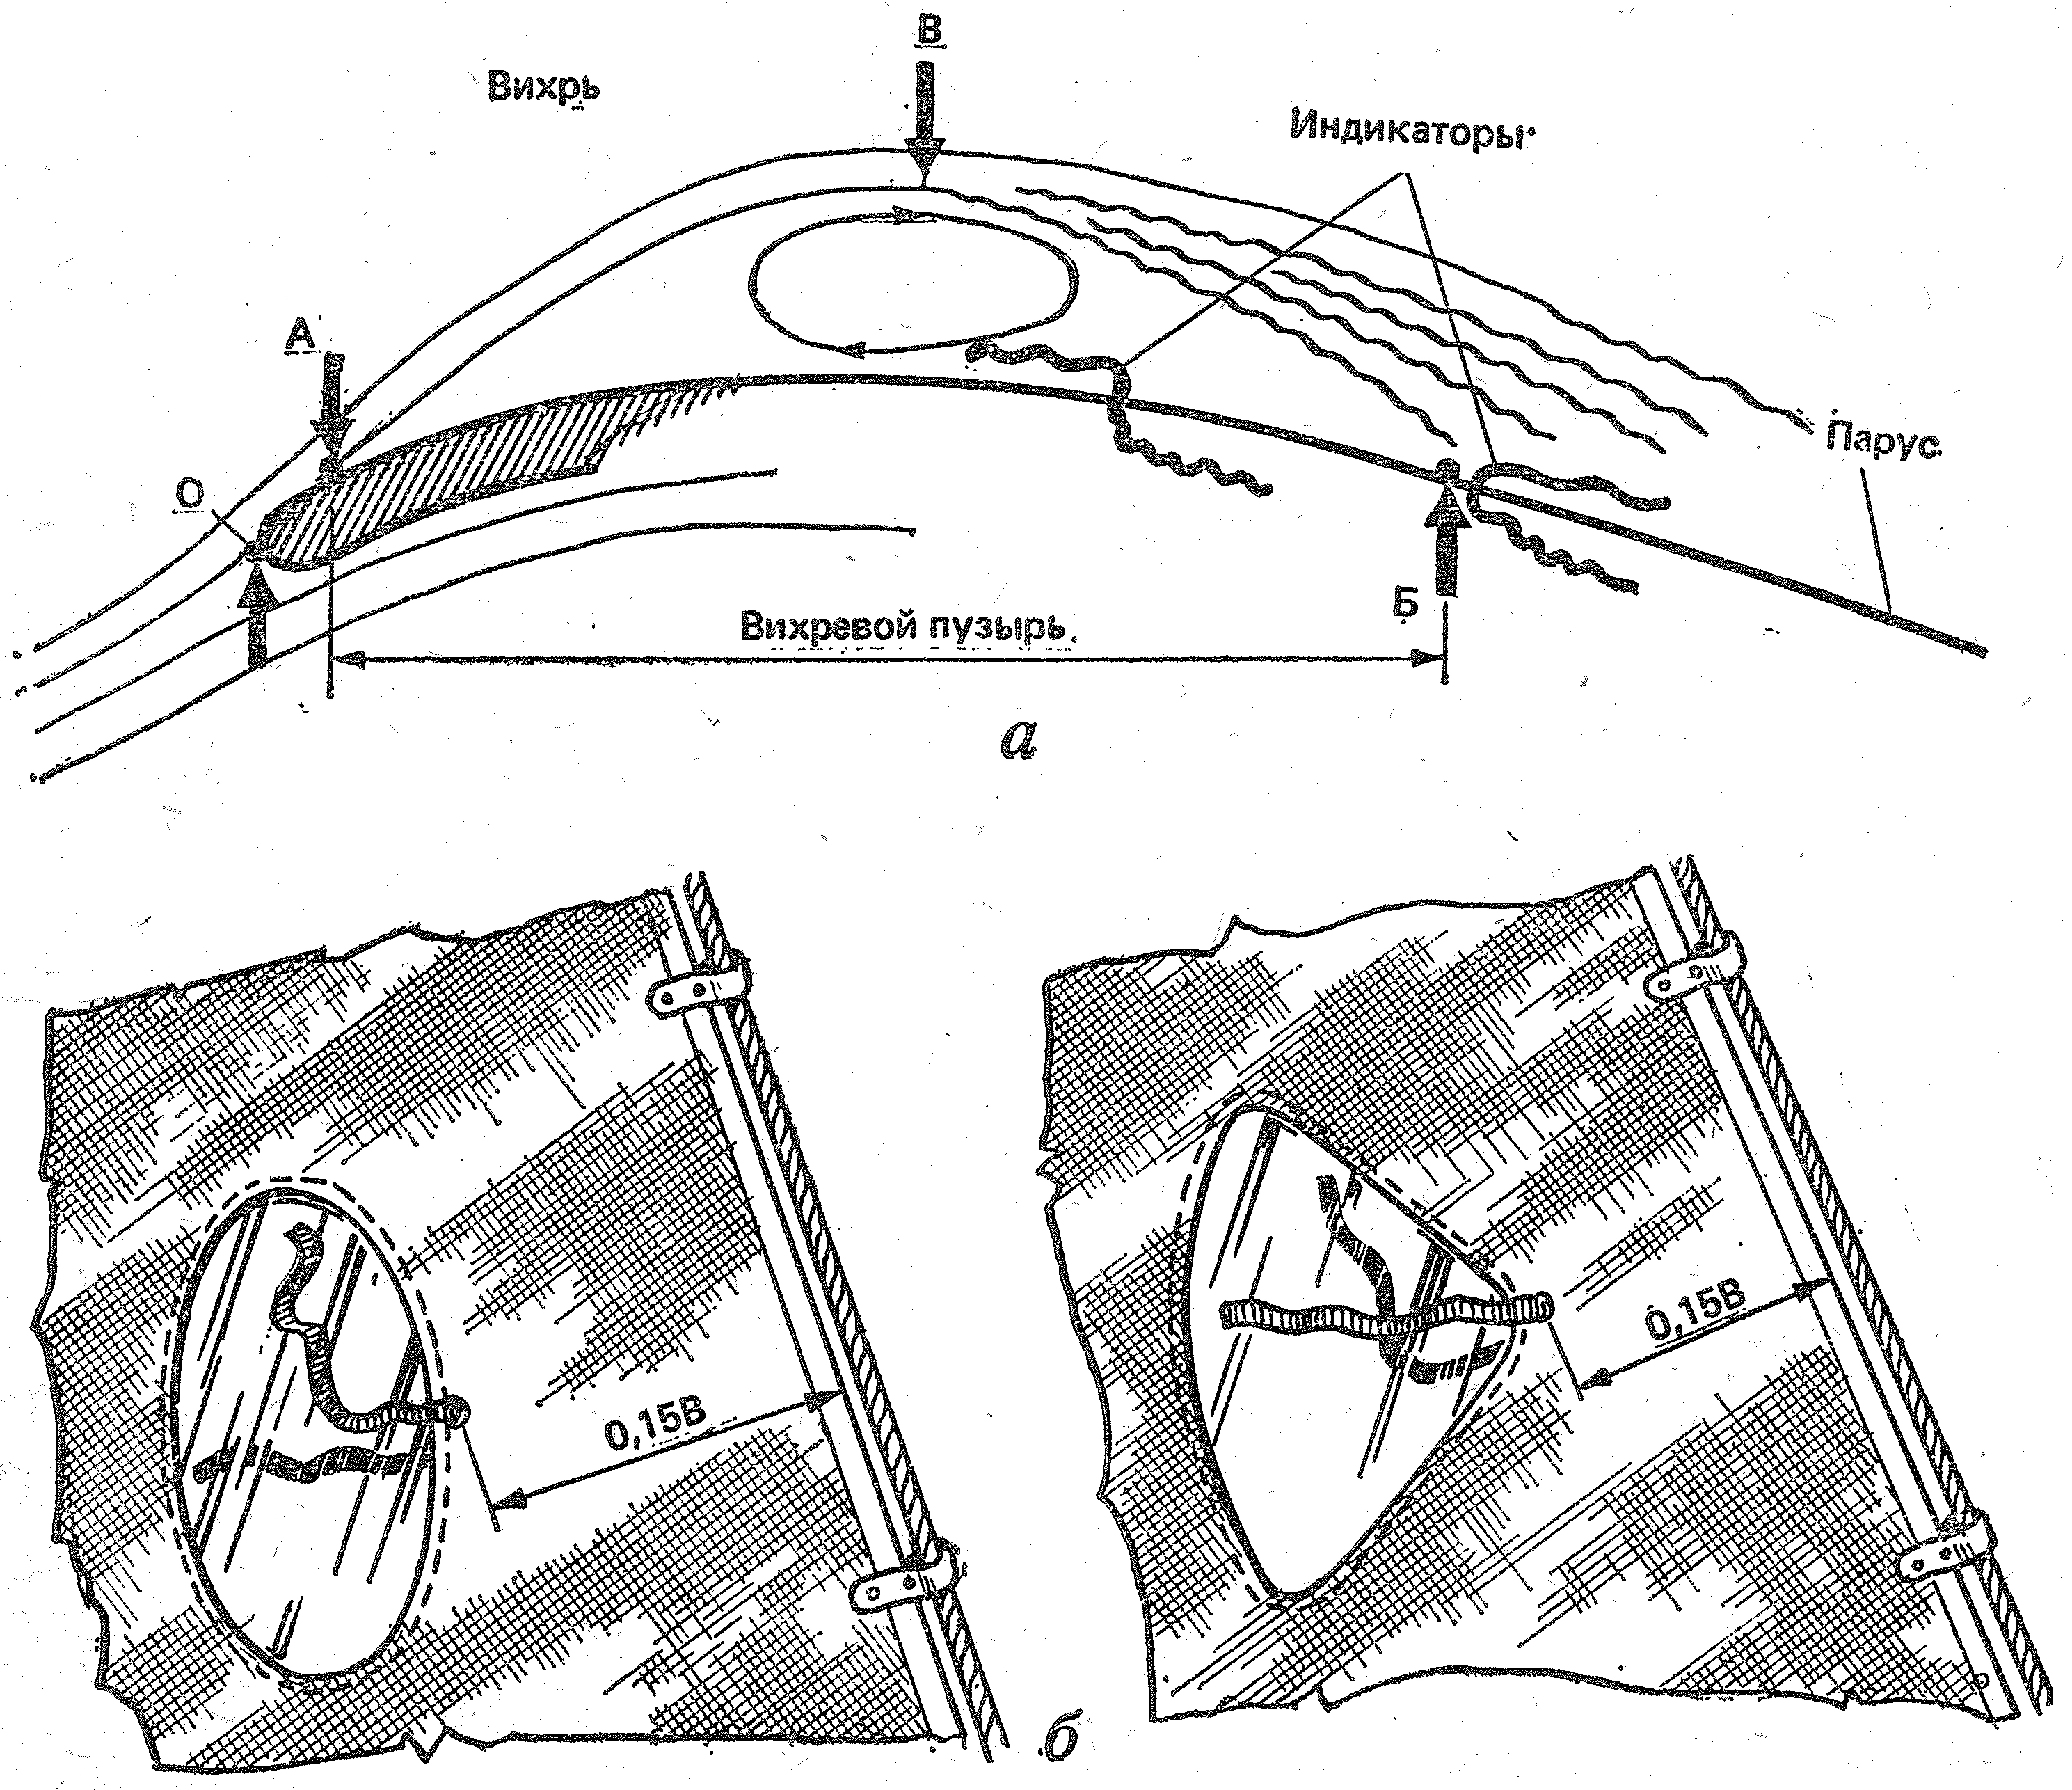
\includegraphics[scale=1.3]{0022P}
  \caption{Принцип работы (\textit{а}) и установка индикаторов обтекания на стакселе (\textit{б})}
  \label{fig:22}
  \small
  \centering{}
  О \--- критическая точка; А \--- точка отрыва пограничного слоя; Б \--- точка возврата пограничного слоя; В \--- переход ламинарного режима потока в турбулентный
\end{figure*}

Таким местом является точка Б возврата пограничного слоя к поверхности паруса. При угле атаки $\alpha = 5\gr$ она отстоит от передней шкаторины примерно на 15\,\% ширины паруса в каждом его поперечном сечении. Как только вихревой пузырь достигнет этой точки, ленточка индикатора на подветренной поверхности паруса, ранее направленная назад по потоку воздуха, отклонится вверх и вперёд, указывая на возникновение здесь вихрей. Дальнейшее выбирание шкотов \--- увеличение угла атаки \--- не только бесполезно, но даже вредно, так как приводит к большой потере подъёмной силы.

Установка трёх\-/четырёх подобных индикаторов, равномерно распределённых по высоте стакселя, облегчает рулевому правильный выбор курса при лавировке. Выбрав наивыгоднейшим образом шкоты для данного курса, ведут яхту таким образом, чтобы индикаторы на наветренной стороне стакселя слегка подрагивали, а на подветренной были вытянуты в сторону задней шкаторины (рис.~\ris{23}).
 
Причиной падения подъёмной силы на парусе является срыв потока с его подветренной стороны при увеличении угла атаки (что соответствует подбиранию шкотов или уваливанию яхты), поэтому главную роль играют индикаторы, расположенные на подветренной стороне. Если они начинают подниматься и совершать беспорядочные движения, значит, необходимо привести яхту к ветру или потравить шкоты.

Угол атаки, при котором подъёмная сила перестаёт расти, называется критическим углом атаки. Его величина зависит от глубины и формы <<пуза>> паруса, аэродинамического удлинения $\lambda$ (оно для парусов вычисляется так же, как и для килей и рулей), наличия у передней шкаторины мачты или обтекателя штага.

\begin{figure*}[htb]
  \centering
  \includegraphics[scale=1.3]{0023P}
  \caption{Поведение индикаторов в зависимости от угла атаки паруса}
  \label{fig:23}
\end{figure*}

В слабый ветер поток воздуха происходит при меньших углах атаки, чем в сильный. При постановке стакселя перед гротом благодаря повышению скорости потока в зазоре между обоими парусами момент срыва сдвигается в сторону больших углов атак. Обратное действие оказывает мачта, срывающиеся с неё на подветренную сторону паруса вихри способствую срыву потока при меньших угла атаки. 

При увеличении угла атаки сверх критического подъёмная сила падает, одновременно растёт лобовое сопротивление. При $\alpha = 90\gr$ подъёмная сила на парусе не создаётся: он обладает лишь лобовым сопротивлением.

\textbf{Поляра паруса.} Характеристикой аэродинамических качеств паруса является поляра \--- график изменения подъёмной силы в зависимости от лобового сопротивления и угла атаки (рис.~\ris{24}, \textit{а}). Для того чтобы поляру можно было применить к парусу любых размеров, по осям координат откладывают не значения сил, а безразмерные коэффициенты подъёмной силы \cidx{C}{Y} и лобового сопротивления \cidx{C}{X}. Данные для построения поляры получают в результате продувок моделей парусов в аэродинамических трубах. 

\begin{figure}[htb]
  \centering
  \includegraphics[scale=1.2]{0024P}
  \caption{Поляра паруса (\textit{а}) и силы, действующие на парус на курсе галфвинд (\textit{б})}
  \label{fig:24}
\end{figure}

С помощью поляры можно определить величины подъёмной силы и лобового сопротивления, а также их составляющих \--- проекций на направление движения яхты. Опустив, например, из точки поляры, соответствующей углу атаки $\alpha = 20\gr$, перпендикуляр на ось движения яхты, можно найти величину коэффициента силы тяги \cidx{C}{Т} как отрезка прямой \cidx{А}{О}. Длина самого перпендикуляра $AB$ будет не что иное, как коэффициент силы дрейфа \cidx{C}{d}. Умножив численные значения коэффициентов \cidx{C}{Т} и \cidx{С}{d} на площадь паруса $S$ и скоростной напор $(\rho v^2)/2$, можно получить величину соответствующих сил. 

Поляра паруса позволяет определить наивыгоднейший угол установки парусов на данном курсе по отношению к ветру. Максимальная тяга, очевидно, определяется перпендикуляром к оси движения яхты, который одновременно является касательной к поляре. Угол атаки $\alpha = 14\gr$, определяемый точкой касания $C$, будет в данном случае наивыгоднейшим. Соответствующий ему угол установки паруса относительно \textit{ДП} яхты $\delta$ несложно найти, вычтя из курсового угла (по отношению к вымпельному ветру $\beta$ дрейф $\lambda$) и угол атаки $\alpha$ (см. рис.~\ris{19}).

Несложно выполнить аналогичные построения для различных значений курсового угла $\beta$ и определить наивыгоднейшие углы установки паруса и соответствующие им углы атаки. Можно убедиться, что для данного паруса почти на всех острых углах к ветру, вплоть до бакштага, наивыгоднейшие углы атаки близки и находятся в пределах 14\otdo 15\gr.

\textbf{Скручивание паруса.} С выбором оптимального угла атаки паруса связано его свойство скручиваться, т.\=,е. изменять угол атаки по высоте. При выбирании шкотов удаётся контролировать только нижнюю треть паруса; в верхней же части ткань имеет возможность несколько отклоняться на подветер, уменьшая тем самым угол атаки. Если не предусмотреть специальных средств для контроля скручивания паруса, то разность в углах атаки или угол скручивания может достичь 20\gr. А так как парус выбирают, ориентируясь на поведение его верхней части (пока не перестанет заполаскивать ткань у передней шкаторины), то нижняя часть оказывается работающей с избыточными углами атаки. Здесь может произойти срыв потока с подветренной стороны и соответственно упасть подъёмная сила. Следовательно, тяга скрученного паруса оказывается ниже, чем если бы каждое его сечение по высоте имело оптимальный угол атаки. 

Особенно сильно заметно скручивание паруса на полных курсах и при свежем ветре, когда шкоты потравлены и нок гика задирается вверх. При этом верхняя часть паруса уходит под ветер и почти заполаскивает, а нижняя работает под слишком большим углом атаки. 

Для уменьшения скручивания грота на большинстве яхт применяют оттяжки гика, препятствующие задиранию нока вверх, а также проводку гика\-/шкота с одним или двумя поперечными погонами, простирающимися на всю ширину яхты. При смещении ползуна гика\-/шкота к борту яхты тяга шкотов становится почти вертикальной, благодаря чему удаётся держать заднюю шкаторину паруса на острых курсах более тугой. 

Свидетельством правильной регулировки натяжения оттяжки гика может служить одновременное (по всей высоте) заполаскивание ткани у передней шкаторины при потравливании шкота.

Было бы ошибкой считать, что парус вообще не должен иметь скручивания по высоте, т. е. иметь все сечения повёрнутыми относительно гика на один и тот же угол. На крупных яхтах надо учитывать изменение скорости и направления вымпельного ветра по высоте и наличие в верхней части паруса перетекания воздуха из зоны повышенного давления на подветренную сторону. В зависимости от высоты парусности и скорости ветра получается разность в углах атаки от 3\otdo 5\gr в бейдевинд до 10\otdo 12\gr на курсе бакштаг. В таких пределах скручивание паруса допустимо и способствует более эффективной его работе. 

Циркуляция воздуха вокруг крыла (см. рис.~\ris{10}), появляющаяся вместе с аэродинамической силой, вызывает незначительные по скорости поперечные потоки воздуха \cidx{V}{И} у входящей и выходящей кромок. Вследствие перетекания воздуха через кромки у концов крыла эти потоки усиливаются и отклоняют основной поток, набегающий на крыло, так, что угол атаки жёсткого треугольного бермудского паруса по мере приближения к вершине увеличивается и близ фалового угла примерно на 20\,\% превышает угол атаки средней части паруса. Близ гика фактический угол атаки, наоборот, несколько уменьшается.

Таким образом, если бы парус не имел скручивания, то его верхняя часть работала бы при закритических углах атаки и практически не участвовала бы в создании движущей силы. Опытный экипаж постоянно контролирует и регулирует скручивание паруса в зависимости от силы ветра и курса яхты с помощью оттяжки гика и перемещения нижнего блока гика\-/шкота по погону.

\textbf{Влияние мачты.} Мачта является источником образования завихрений, которые особенно неблагоприятно сказываются на формировании потока на подветренной стороне паруса. Здесь вихревой след мачты уменьшает разрежение, вследствие чего уменьшается величина подъёмной силы. Кроме того, сама мачта обладает достаточно большим лобовым сопротивлением. 

\begin{figure}[htb]
  \centering
  \includegraphics[scale=1.2]{0025P}
  \caption{Характер обтекания мачт}
  \label{fig:25}
  \small
  \centering{}
  \textit{а} \--- с эллиптическим поперечным сечением; \textit{б} \--- с параболической передней кромкой; \textit{в} \--- с парусом поставленным по подветренной кромке
\end{figure}

Большую роль играет форма поперечного сечения мачты, особенно передней её кромки, на которой формируется поток. Важно, чтобы на курсе бейдевинд, когда яхта идёт под углом 25\otdo 30\gr к вымпельному ветру, вихревая дорожка, срывающаяся с подветренной стороны мачты, имела бы минимальную ширину. Парус за мачтой параболическим поперечным сечение и тупой кормовой кромкой обладает более высоким аэродинамическим качеством, чем за мачтой эллиптического сечения (рис.~\ris{25}). Наиболее оптимальным оказывается вариант мачты с парусом, закреплённым передней шкаториной близ её подветренной стороны: качество его работы на 40\,\% выше, чем паруса с эллиптической мачтой. Это лишнее свидетельство тому, что отрицательное влияние мачты в основном распространяется на подветренную сторону паруса.

Мачта, имеющая большое поперечное сечение, может снизить подъёмную силу паруса на 25\,\% по сравнению с парусом, поставленным на штаге. Особенно велики потери подъёмной силы при постановке паруса на рельсе с ползунками, когда в щель между мачтой и парусом перетекает воздух с наветренной стороны паруса в область пика разрежения на подветренной стороне. Неудачны мачты цилиндрического сечения, без сужения к топу: в верхней части отношение диаметра мачты уменьшающейся здесь ширине пару становится велико. Может оказаться, что часть паруса близ фалового угла вообще не будет участвовать в создании подъёмной силы, а следовательно, и тяги на курсе бейдевинд.

Наибольшее распространение на яхтах получили мачты, имеющие овальное поперечное сечение, с соотношением около 3:2, обеспечивающее большую продольную жёсткость. Каплевидные и другие типы обтекаемых профилей целесообразны только в том случае, если мачта вращается для установки под наивыгоднейшим углом к вымпельному ветру при перемене галса. Такими мачтами снабжают обычно буера и катамараны.

\section{Форма паруса и контроль за нею}

\begin{figure}[htb]
  \centering
  \includegraphics[scale=1.2]{0026P}
  \caption{Влияние <<пуза>> паруса на величину подъёмной силы и лобового сопротивления}
  \label{fig:26}
\end{figure}

\textbf{Поперечный профиль паруса.} Основным фактором, влияющим на величину аэродинамических сил на парусе и его тяговые характеристики, является его профиль, т.\=,е. форма и размеры <<пуза>>.

На рис.~\ris{26} представлены поляры четырёх жёстких моделей бермудских парусов, имеющих аэродинамическое удлинение $\lambda = 4$ и расстояние максимальной глубины <<пуза>> от передней шкаторины, равное 1/3 хорды. От реальных парусов модели отличались ещё отсутствием угла скручивания и постоянством относительной глубины <<пуза>> по высоте.

На полярах (рис.~\ris{26}) видно, что с уменьшением глубины <<пуза>> качество паруса возрастает благодаря снижению коэффициента лобового сопротивления (показано горизонтальной стрелкой). Максимальная подъёмная сила паруса, наоборот, увеличивается по мере увеличения глубины <<пуза>> (показано наклонной стрелкой).

Посмотрим теперь, каким образом могут быть реализованы качества парусов в зависимости от их профиля. Предположим, что яхта идёт курсом бейдевинд под углом $\beta = 30\gr$ к направлению вымпельного ветра. Очевидно, наибольшую тягу даст тот парус, касательная к поляре которого \--- перпендикуляр к линии пути яхты (см. рис.~\ris{24}) будет отстоять от точки 0 дальше подобных же касательных к другим полярам. В данном случае наибольшую тягу имеет парус с относительной глубиной <<пуза>> $f/b=1/10$. Однако нетрудно заметить, что выигрыш в тяге этого паруса будет минимальным по сравнению с более плоским парусом, имеющим $f/b = 1/15$. В то же время, более <<пузатый>> парус ($f/b = 1/10$) даёт значительно большую поперечную силу дрейфа, чем парус с $f/b = 1/15$. Поэтому небольшое преимущество более <<пузатого>> паруса может быть реализовано на лавировке только в слабый ветер, когда абсолютная величина силы дрейфа будет невелика. В свежий ветер плавание с таким парусом сопровождается большим креном и соответственно дополнительным сопротивлением движению, так что в конечном счёте выигрыша в скорости не получится. 

Ещё более <<пузатые>> паруса $f/b=1/5$ и $f/b=1/4$ на курсе бейдевинд не только не дают увеличения силы тяги, но и отличаются намного большей величиной силы дрейфа. Однако более высокий коэффициент подъёмной силы <<пузатых>> парусов может быть реализован на других, более полных, курсах по отношению к ветру: например, на курсе галфвинд, когда подъёмная сила даёт наибольшую составляющую на направление движения (см. рис.~\ris{24}, \textit{б}). В практике морских гонок это качество <<пузатых>> парусов используется благодаря смене на полных курсах лавировочных передних парусов на дрифтергеную, блупер или спинакер.

Следует заметить, что преимущества <<пузатых>> парусов могут быть использованы в основном при слабых ветрах, когда скорость яхты прямо пропорциональна силе тяги. В сильные ветра, когда яхта развивает свою предельную скорость под обычными лавировочными парусами и дальнейшее повышение тяги практически не увеличивает скорость, постановка <<пузатых>> парусов не даёт эффекта. Более того, большая сила дрейфа <<пузатого>> паруса обусловливает больший крен и дрейф и соответствующее повышение сопротивления воды движению яхты. 

В качестве основных (лавировочных) парусов для среднего ветра (2\otdo 4 балла) применяют паруса с <<пузом>> $f/b=9\motdo 10\,\%$. Для слабого ветра выгодны более <<пузатые>> паруса \--- $f/b$ до 12\,\%, а при ветре более 5 баллов \--- паруса с <<пузом>> не более 6\,\% ($f/b=1/17\motdo 1/25$). 

В гонках яхтсмены широко пользуются различными способами регулирования величины <<пуза>> парусов в зависимости от силы ветра. Особенно это относится к настройке грота, так как по правилам IOR замена его во время гонок не допускается, а ветровые условия могут изменяться в довольно широких пределах. Основными средствами регулирования <<пуза>> грота являются продольный изгиб мачты, натяжение шкаторин (оттяжка Кэнингхэма и грота\-/шкот), уплощающий риф, натяжение гика\-/шкота и положение его блока на погоне по ширине яхты, оттяжка гика. Продольный изгиб мачты позволяет контролировать две верхние трети паруса, в то время как другие средства эффективны при изменении профиля у гика.

В слабый ветер, когда важно иметь грот наиболее <<пузатым>>, мачта должна быть прямой, грота\-/шкот и оттяжку гика выбирают не до конца, оттяжка Кэнингхэма растравлена. Блок на погоне гика\-/шкота перемещают от \textit{ДП} в сторону наветренного борта; гика\-/шкот втугую не выбирают.

Для увеличения <<пуза>> стакселя или генуи блок (кипу) стаксель\-/шкота перемещают вперёд и ближе к \textit{ДП} яхты. При этом <<пузо>> перемещается вперёд, натяжение задней шкаторины ослабляется, зазор между гротом и стакселем увеличивается. 

С усилением ветра мачте придают изгиб с выпуклостью, направленной вперёд, увеличивая натяжение ахтерштага (при оснастке типа 3/4 или 7/8) или регулируя натяжение промежуточного штага и бакштагов (при топовой оснастке). Благодаря этому излишек паруса убирается в образовавшийся серп у передней шкаторины, <<пузо>> становится меньше и перемещается ближе к мачте. Оттяжку Кэнингхэма, грота\-/шкот и оттяжку гика выбираю втугую; блок гика\-/шкота смещают по погону на подветренный борт. Шкоты выбирают более туго, чем в слабый ветер. При необходимости сделать парус ещё более плоским в нижней части берут уплощающий риф, используя люверсы, расположенные вблизи гика.

Профиль генуи может быть сделан более плоским при передвижении блока стаксель\-/шкота назад и к борту большем натяжении передней шкаторины. Значительное влияние на профиль передних парусов оказывает натяжение штага: для того чтобы парус стал более плоским, необходимо по возможности ликвидировать прогиб штага.

Большое влияние на тяговые характеристики паруса кроме величины <<пуза>> оказывает место положения максимальной выпуклости от передней шкаторины. На рис.~\ris{27} показано распределение разрежения на подветренной стороне жёсткой модели паруса с относительной величиной <<пуза>> $f/b = 0,188$ при отстоянии максимального <<пуза>> на 40 и 60\,\% хорды от передней кромки и при угле атаки $\alpha = 15\gr$ (характерный <<провал>> на эпюре давления являйся следствием развитого вихревого пузыря \--- см. рис.~\ris{21}). Как видим, в создании движущей силы главную роль играет передняя часть паруса, где концентрируется разрежение у паруса с <<пузом>>, расположенным на 40\,\% хорды от передней шкаторины. Когда же <<пузо>> смещено к задней шкаторине, область разрежения охватывает и заднюю часть профиля, вследствие чего увеличивается составляющая \ve R, направленная против движения яхты. Таким образом, при смещении <<пуза>> к задней шкаторине эффективность паруса снижается как в результате падения подъемной силы в передней части паруса, так и в результате роста сил сопротивления, тормозящих ход судна.

\begin{figure}[htb]
  \centering
  \includegraphics[scale=1.2]{0027P}
  \caption{Эффект распределения разрежения на подветренной стороне паруса на результирующую аэродинамическую силу на парусе}
  \label{fig:27}
  \small
  \centering{}
  \textit{а} \--- эпюра распределения разрежения; \textit{б} \--- силы на парусе; \textit{1} \--- парус с максимальным <<пузом>>, расположенным на расстоянии $0,4 b$ от передней шкаторины; \textit{2} \--- парус с <<пузом>>, расположенным на $0,6 b$ от передней шкаторины. $ем Y_1$ и $\ve Y_2$ \--- подъёмная сила; \ve T и \ve R \--- составляющие силы \ve A по направлению ветра
\end{figure}

Лавировочные паруса шьют с максимальной глубиной <<пуза>>, расположенной от передней шкаторины на расстоянии от 35\otdo 40\,\% ширины паруса $b$ для плоских парусов, до 40\otdo 50\,\% $b$ для более полных.

Во всех поперечных сечениях максимальная глубина <<пуза>> должна находиться в указанных пределах. Поэтому по мере увеличения ширины паруса по направлению к гику соответственно увеличивается и абсолютная величина <<пуза>>. У гика на обезветренном парусе <<пузо>> образует <<мешочек>>, который в сильный ветер можно убрать в скатку уплощающего рифа.

\textbf{Форма паруса.} С точки зрения аэродинамики крыла наиболее выгодным был бы парус с эллипсовидной верхней частью. Именно в его верхней части образуются потоки воздуха, перетекающего с наветренной стороны на подветренную \--- в область разрежения. В результате возникают вихри, срывающиеся с кромки паруса и уходящие в пространство. Эти возмущения требуют затрат кинетической энергии ветра, которые выражаются в росте общего аэродинамического сопротивления судна в виде составляющей индуктивного сопротивления. 

\begin{figure}[htb]
  \centering
  \includegraphics[scale=1.2]{0028P}
  \caption{Поляры парусов с различным аэродинамическим удлинением}
  \label{fig:28}
\end{figure}

Очевидно, что наибольшим индуктивным сопротивлением обладает четырёхугольный гафельный парус, у которого перетекание воздуха происходит по верхней и нижней широким кромкам. Поэтому коэффициент подъёмной силы здесь резко падает (см. рис.~\ris{8}).

У паруса с эллипсовидной верхней частью величина подъёмной силы из-за плавного уменьшения площади паруса у верхнего конца также плавно убывает. Благодаря этому плавно убывает и интенсивность перетекания воздуха через кромки, не происходит местного изменения угла атаки и коэффициента подъёмной силы. 

Попытка приблизить форму паруса к эллипсовидной при существующих ограничениях ширины фаловой доски и эластичности мачты была сделана, например, на английском двенадцатиметровике <<Лайонхат>> \--- претенденте на Кубок Америки 1980\,г.: верхняя часть мачты на нем была сильно изогнута. Испытания в аэродинамической трубе показали, что грот с гнутой мачтой даёт примерно 10\otdo 30\,\% увеличения движущей силы по сравнению с обычным бермудским парусом или увеличение скорости лавировки на ветер порядка 4\,\%.
 
У треугольного паруса основная площадь и, следовательно, нагрузка сосредоточены в нижней трети. По мере приближения к фаловому углу площадь и подъёмная сила убывают, что сопровождается соответствующим уменьшением скорости и фактического угла атаки паруса к набегающему потоку. Близ фалового угла также усиливается отрицательный эффект мачты поскольку размеры её сечения увеличиваются относительно хорды паруса. Эксперименты показали, что если срезать бермудский парус на 15\,\% высоты от вершины, то практически его тяга не уменьшится. 

Существенное влияние на характеристики паруса оказывает аэродинамическое удлинение паруса (отношение длины передней шкаторины) к его средней хорде, измеренной на половине высоты, или отношение квадрата высоты паруса и его площади.

На рис.~\ris{28} представлены поляры трёх парусов различного удлинения --- от $\lambda = 1$ до 6, имеющих одинаковое <<пузо>> $f/b=7,4\,\%$. Сравнивая поляры можно заметить, что при угле атаки $\alpha = 10\gr$ наивысшую аэродинамическу силу дает парус с максимальным удлинением $\lambda = 6$. Этот же парус имеет наивыгоднейшее направление аэродинамической силы для получения максимальной тяги на курсе бейдевинд. 

Аэродинамическая сила на парус имеющем $\lambda = 6$ достигает максимум при $\alpha = 15\gr$, затем падает. При угле атаки около 35\gr, т. е. на полных курсах, заметное преимущество получай более широкие паруса, имеющие $\lambda = 1$. Таким образом, можно сделать вывод, что парус с большим удлинением при переходе яхты на полный курс становится менее выгодным. На курсе полный бакштаг, например, более быстроходной может оказаться яхта, оснащённая широкими гафельными парусами с удлинением около 1. Вот почему несмотря на общепризнанное преимущество бермудских парусов, гафельные паруса довольно часто применяют на моторно-парусных яхтах, у которых паруса используются преимущественно при сильных ветрах и на попутных курсах. 

У большинства современных яхт лавировочные паруса имеют отношение длин шкаторин от 3 до 5; паруса для полных курсов \--- дрифтеры, блуперы и спинакеры шьют с соотношением шкаторин, близким к 1.

Пределом для использования парусов большого удлинения является ограниченная остойчивость яхт, не позволяющая чрезмерно повышать положение \textit{ЦП}. Более высокая парусность требует также рангоута большего сечения, что приводит к распространению влияния мачты на большую часть площади грота.

\section{Взаимодействие парусов}

Мы рассматривали особенности \--- аэродинамики одиночного паруса как крыла с тонким поперечным профилем. Большинство яхт, однако, оснащены по крайней мере двумя парусами \--- гротом и стакселем. Поскольку оба паруса расположены в непосредственной близости друг от друга и обтекаются одним потоком воздуха, то естественно предположить наличие их взаимного влияния. 

\begin{figure}[htb]
  \centering
  \includegraphics[scale=1.2]{0029P}
  \caption{Взаимодействие грота и стакселя}
  \label{fig:29}
  \small
  \centering{}
  \textit{а} \--- циркуляция потока вокруг обоих парусов; \textit{б} \--- влияние отклонения потока, натекающего на грот и стаксель под действием циркуляции; $\ve Y_C$ и $\ve Y_T$ \--- подъёмные силы на стакселе и гроте, работающих как изолированные паруса; $\ve Y_1$ и $\ve Y_2$ \--- подъёмные силы на парусах, работающих совместно; $\ve V_1$ и $\ve V_2$ \--- скорости, вызванные циркуляцией потока вокруг обоих парусов
\end{figure}

До недавнего времени среди яхтсменов пользовалась популярностью теория Вентури, заимствованная из авиации. Согласно этой теории, основным назначением стакселя считалось создание щели \--- сопла между стакселем и гротом, входя в которую, поток воздуха увеличивает свою скорость, способствуя тем самым понижению давления на подветренной стороне грота, особенно в районе, где паруса перекрывают друг друга. В результате должна увеличиваться аэродинамическая сила на гроте.

В настоящее время взаимодействие парусов рассматривается на основании вихревой теории крыла \--- исходя из наличия циркуляции вокруг обоих парусов (рис.~\ris{29}). Основная роль в паре грот \--- стаксель принадлежит стакселю. Бесспорно, что воздух, протекающий в щели между гротом и стакселем, имеет повышенную скорость. Однако это прежде всего сказывается на скорости потока, обтекающего подветренную сторону стакселя. Частицы воздуха, вырываясь из щели, увлекают с собой воздух с подветренной стороны стакселя подобно эжектору. Соответственно ускоряется поток вдоль всей подветренной поверхности стакселя, увеличивается циркуляция вокруг его профиля и возрастает аэродинамическая сила. И что ещё важно - парус может работать без срыва потока на больших углах атаки.
 
Вызванная скорость (поперечная составляющая вследствие циркуляции) у передней шкаторины грота увеличивает угол атаки, под которым поток натекает на стаксель. Благодаря этому аэродинамическая сила растёт и отклоняется вперёд \--- на более выгодный угол. На курсе бейдевинд, к слову сказать, большой генуэзский стаксель даёт на 30\,\% большую движущую силу, чем грот, и на 45\,\% меньшую силу дрейфа.
 
Грот работает в области потока, отклоняемого вызванными скоростями у задней шкаторины стакселя. Это приводит к уменьшению угла атаки грота. Однако воздух, отражённый от стакселя, как бы прилипает к подветренной поверхности грота, благодаря чему предотвращается отрыв от неё пограничного слоя.

Стаксель влияет и на положение критической точки: она перемещается с наветренной стороны мачты ближе к её передней кромке. В результате уменьшается скорость потока с подветренной стороны грота и сильно снижается пик разрежения у передней шкаторины. Поэтому тенденция к отрыву пограничного слоя и образованию завихрений на гроте ослабевает, парус более эффективно работает на больших углах атаки, чем без стакселя. Скорее этим, а не ускорением потока в щели между гротом и стакселем, по теории Вентури, можно объяснить положительное действие стакселя на работу грота.

Чем больше выбирают стаксель, тем меньше становится разность давлений на подветренной и наветренной сторонах грота. Когда они сравняются, выпуклая форма паруса уже не может поддерживаться \--- парус заполаскивает. Поскольку стаксель более эффективен, чем грот, и даёт меньшую кренящую силу, то экипажи крейсерско\-/гоночных яхт уделяют большое внимание подбору стакселей для различных курсов и силы ветра. В гонках при усилении ветра целесообразно уменьшат площадь парусности рифлением грота продолжая по возможности нести стаксель. На отдельных порывах крен можно уменьшать, потравливая грот.

Поскольку Правила обмера IOR прямо не ограничивают длину нижней шкаторины стакселей, то обычно стараются шить их с максимальным перекроем (заходом стакселя за мачту). Существуют, однако, вполне определённые пределы перекроя, далее которых парус теряет свою эффективность и начинает отрицательно влиять на работу грота.

Прежде всего это обеспечение оптимального угла установки стакселя относительно ДП яхты, который равен для лавировки 12\otdo 18\gr. Это труднодостижимо при большой длине нижней шкаторины стакселя и сравнительно небольшой ширине палубы яхты. Как правило, кипы стаксель\-/шкотов удаётся разместить при несколько меньших углах установки паруса \--- 9\otdo 12\gr. По этому при слишком <<пузатом>> стакселе возможен сток потока воздуха с него на переднюю шкаторину грота и заполаскивание её по всей высоте. Кроме того, возможно сильное скручивание стакселя: в верхней части ветер будет выдувать из паруса и он перестанет работать. 

\begin{figure}[htb]
  \centering
  \includegraphics[scale=1.2]{0030P}
  \caption{Оттяжка шкотового угла стакселя}
  \label{fig:30}
\end{figure}

Для регулирования положения кип стаксель\-/шкотов в зависимости от величины стакселя и курса относительно ветра используют специальный фальшборт из металлического угло\-/бульбового профиля с большим числом отверстий или крепят кипы на передвижных ползунах, скользящих по прочному палубному рельсу. При настройке стакселя стараются получить равномерный зазор между гротом и стакселем по всей высоте и <<пузо>> стакселя, смещённое к передней шкаторине. При перемещении кипы вперёд тяга шкота сильнее натягивает заднюю шкаторину. В результате <<пузо>> увеличивается по всей площади, парус меньше скручивается, но возможно заворачивание задней шкаторины на ветер. При перемещении кипы назад, увеличивается натяжение нижней шкаторины; натяжение задней шкаторины будет недостаточным, парус сильно скрутится и может заполаскивать в верхней части. Иногда полезно применить дополнительную снасть \--- оттяжку шкота (рис.~\ris{30}) для осаживания задней шкаторины. Выбрав втугую парус по нижней шкаторине за шкот, с помощью оттяжки добиваются нужного натяжения задней шкаторины и положения <<пуза>> по ширине паруса, устраняют сильное скручивание. Правильно отрегулированный стаксель должен давать поток воздуха, направленный по касательной к поверхности грота и при приведении яхты заполаскивать сразу по всей высоте. Хорошую службу при настройке могут оказать индикаторы (см. рис.~\ris{22}--\ris{23}).

Большое влияние на полноту стакселя оказывает прогиб штага. Чем сильнее при усилении ветра прогибается штаг, тем больше становится <<пузо>> паруса и он начинает задувать на грот. В известной мере прогиб компенсируется специальным раскроем стакселя с выпуклостью в нижней части передней шкаторины и вогнутостью (отрицательным серпом) в верхней. Многие яхты за рубежом снабжают мощными гидравлическими, винтовыми устройствами или талями для увеличения натяжения ахтерштага и даже наклона мачты назад.

\section{Лобовое сопротивление яхты}

Влияние лобового (воздушного) сопротивления яхты на её ходовые качества исключительно велико. На курсе бейдевинд при ветре 4 балла на преодоление воздушного сопротивления яхты затрачивается около одной трети силы тяги, развиваемой парусами. Поэтому снижение лобового сопротивления так же важно, как и снижение сопротивления воды.

В общем балансе воздушного сопротивления на долю парусов и рангоута приходится 70\otdo 78\,\%, такелажа \--- 3\otdo 5\,\%, корпуса \--- 15\otdo 18\,\%, экипажа \--- 4\otdo 6\,\%. Поскольку основную роль играют паруса и рангоут, рассмотрим причины, обусловливающие появление на них сил сопротивления.

Воздушное сопротивление, как и сопротивление воды, считают возможным разделить на несколько компонентов. Для парусов их два: индуктивное сопротивление и сопротивление формы (или профильное). Как мы уже говорили, индуктивное сопротивление является неизбежным следствием действия на парусе аэродинамической подъёмной силы. По мере роста скорости вымпельного ветра и соответственно величины подъёмной силы растёт и величина индуктивного сопротивления. В средний ветер в области оптимальных углов атаки паруса ($\alpha = 5\motdo 15\gr$) индуктивное сопротивление существенно выше сопротивления формы. Проявляется оно в виде двух вихревых дорожек, стекающих с нижней шкаторины и близ фалового угла паруса.
 
Основные факторы, влияющие на индуктивное сопротивление, \--- аэродинамическое удлинение и форма парусов, угол скручивания и распределение <<пуза>> по высоте паруса. Чем больше удлинение паруса (т.\=,е. чем меньше относительно высоты паруса длина нижней шкаторины и верхней части паруса, через которые происходит перетекание воздуха из зоны повышенного давления на сторону разрежения), чем ближе к форме эллипса форма верхней части паруса, тем меньше индуктивное сопротивление. От угла скручивания и величины <<пуза>> в верхней части паруса зависит величина подъёмной силы и её распределение на этом участке. У треугольного бермудского паруса в верхней части желательно получить большую подъёмную силу на единицу площади, чем на середине высоты мачты, потому что тогда характер распределения нагрузки приближается к эллиптическому крылу, имеющему минимальное индуктивное сопротивление. Вот почему в верхней части паруса часто выкраивают с несколько большим <<пузом>>, а скручивание паруса допускается лишь на незначительные углы. Корпус яхты, в непосредственной близости от которого располагаются нижние шкаторины парусов, является своеобразной аэродинамической шайбой, в известной мере снижающей перетекание воздуха через нижние шкаторины. 

Профильное сопротивление парусов, в свою очередь, можно разделить на сопротивление трения и давления. Сопротивление трения вызвано вязкими свойствами воздуха и подчиняется тем же законам, что и сопротивление трения воды, хотя коэффициент кинематической вязкости воздуха в 860 раз меньше, чем воды. Нормальным режимом обтекания парусов является турбулентный, при котором коэффициент сопротивления трения в большой степени зависит от степени гладкости поверхности. Более ворсистые и имеющие крупную текстуру хлопчатобумажные ткани обладают большим сопротивлением трения, чем лавсановые или дакроновые, особенно пропитанные смолой. 

Сопротивление трения повышается при наличии на парусах большого количества швов, поперечных морщин складок, различных нашивок. Особенно важно иметь гладкую поверхность близ передней шкаторины паруса, где возможно ламинарное обтекание и где формируется поток вдоль подветренной стороны паруса. Наличие здесь морщин или нашивок способствует турбулизации потока и его отрыву от поверхности паруса, в результате чего падает подъёмная сила. 

Сопротивление давления зависит от формы поперечного сечения \--- профиля паруса и угла атаки его относительно вымпельного ветра. Очевидно, что сопротивление плоской пластины при нулевом угле атаки во флюгерном положении будет полностью обусловлено трением. По мере увеличения угла атаки появится дополнительное сопротивление, которое при расположении пластины перпендикулярно потоку будет максимальным и полностью представит собой сопротивление давлений. Если при $\alpha = 0\gr$ коэффициент сопротивления пластины $C_X = 0,004\motdo 0,008$, то при $\alpha = 90\gr$ $C_X = 1,9$. Это означает, что сопротивление давления может в 250\otdo 500 раз превышать сопротивление трения, однако влияние трения на режим обтекания паруса и его подъёмную силу заставляет парусных мастеров экипажа яхты уделять качеству отделки парусов достаточно большое внимание.

Сопротивление давления паруса, имеющего <<пузо>>, при малых углах атаки превышает сопротивление плоской пластины. Чем больше относительная величина <<пуза>> и чем дальше передней кромки оно располагается, тем больше профильное сопротивление. На его величине сильно сказываются искажения правильного профиля \--- складки, слишком туго набитые в карманах латы, свободно болтающаяся или, наоборот, слишком перебранная задняя шкаторина и т.\=,п.
 
О вредном, но неизбежном влиянии мачты на тяговые характеристики паруса мы уже говорили. Кроме того, мачта сама по себе является далеко не идеально обтекаемым телом, обладает довольно значительным профильным сопротивлением, которое возрастает с увеличением скорости ветра. Немало случаев, когда в сильный попутный ветер яхта под одним рангоутом развивает достаточную скорость, чтобы слушаться руля.

Иное дело обтекатели штага, снабжённые ликпазом, которые в последнее время все чаще находят применение на крейсерско\-/гоночных яхтах (см. рис.~\ris{46}). Выполняемые обычно в виде хорошо обтекаемого алюминиевого или пластикового профиля с толщиной, равной 24\otdo 29\,\% хорды, они примерно на 20\,\% снижают профильное сопротивление стакселя и на 5\,\% повышают его подъёмную силу. Главный эффект состоит в оформлении и утолщении входящей кромки стакселя как аэродинамического профиля. Критическая точка (см. рис.~\ris{22}) перемещается ближе к подветренной стороне обтекателя, благодаря чему пик разрежения вблизи передней шкаторины становится плавнее и достигается при несколько больших углах атаки. Кроме того, обтекатели способствуют уменьшению прогиба штага, отрицательно влияющего на профиль паруса.

В отличие от сопротивления паруса, создающего движущую силу, сопротивление мачты, краспиц, гика, стоячего и бегучего такелажа относят к так называемому паразитному сопротивлению. Оно занимает 10\otdo 12\,\% общего воздушного сопротивления, поэтому сокращение длины и уменьшение диаметра всех тросов на яхтах очень важно. Мачты желательно <<очистить>> от большинства фалов и электропроводки, убрав их внутрь. По возможности внутри мачты следует расположить крепления стоячего такелажа и блоки фалов.

\section{Ходовые качества яхты на различных курсах}

\begin{figure}[htb]
  \centering
  \includegraphics[scale=1.2]{0031P}
  \caption{Полярная диаграмма скорости яхты}
  \label{fig:31}
\end{figure}

Появившиеся в оснащении яхт приборы позволяют измерять параметры их движения и на основе этих измерений оценивать ходовые качества судна на разных курсах по отношению к ветру количественно, а не <<на глазок>>. Наиболее доступные приборы дают следующую информацию:

\begin{itemize}
\item угол между \textit{ДП} яхты и направлением вымпельного ветра; 
\item скорость вымпельного ветра; 
\item скорость яхты относительно воды; 
\item мгновенное изменение скорости яхты относительно выбранной точки отсчёта. 
\end{itemize}

Пользуясь показаниями этих приборов, экипаж может оптимальным образом настроить паруса для каждого курса, чтобы получить наивысшую скорость, а также построить полярную диаграмму ходкости яхты (рис.~\ris{31}). При построении диаграммы яхта считается расположенной в центре нескольких концентрических окружностей, каждая из которых соответствует определённой скорости (4, 5, 6 и т.\=,д. уз). Из центра через 10\gr проводятся лучи, обозначающие курсы яхты по отношению к направлению истинного (или вымпельного) ветра. Для удобства в правой части диаграммы могут быть нанесены курсы судна относительно направления истинного, а по левую \--- относительно вымпельного ветра. Затем на каждом луче откладывается значение оптимальной скорости на данном курсе и при данной силе ветра.

Нетрудно заметить, что поляра скорости яхты на курсе от полного бейдевинда до крутого бакштага близка к дуге окружности, иными словами, с изменением курсового угла ветра скорость меняется очень незначительно. При переходе яхты на чистый фордевинд скорость заметно падает, особенно в слабый ветер. Объясняется это существенным снижением скорости вымпельного ветра и, поскольку аэродинамические силы пропорциональны её квадрату, уменьшением силы тяги.

Постановка дополнительных парусов \--- спинакера и блупера помогает увеличить скорость яхты в слабый и средний ветер. В сильный же ветер, когда скорость оказывается близкой к предельной, $v = 3 \cdot {\lkvl}^{1/2}$, уз. и кривая сопротивления воды круто поднимается вверх, увеличение силы тяги при увеличении парусности практически не даёт повышения скорости. На курсе бейдевинд скорость вымпельного ветра и аэродинамические силы максимальные, однако подъёмная сила даёт очень небольшую составляющую в направлении движения яхт (см. рис.~\ris{20}). С увеличением же на этом курсе крена уменьшается эффективный угол атаки относительно вымпельного ветра, падает величина аэродинамической силы и силы тяги. По этому на острых курсах более остойчивая яхта может оказаться быстроходней. 

С помощью полярной диаграммы рулевой яхты может решать различные тактические задачи, например выбрать оптимальный курс в лавировку. Он определяется по наибольшей скорости продвижения прямо против ветра. Для этого следует провести касательную к поляре для данной силы ветра \--- перпендикуляр к его направлению. Точка касания поляры указывает наиболее выгодный курс. При плавании полным курсом, зная расстояние до конечной точки, можно с помощью поляры определить, как выгоднее будет пройти дистанцию \--- курсом фордевинд или двумя бакштагами со сменой галса.

Для того чтобы облегчить возможность использования полярной диаграммы, на кривых скорости наносят курсы яхты относительно вымпельного ветра. Получаются они построением треугольника скоростей по данным снятым с диаграммы (см. рис.~\ris{19}, \textit{б}) поскольку с движущейся яхты определить направление истинного ветра можно только приближённо \--- с помощью компаса и волны либо по береговым приметам.
